\subsection{OoS KS Test-Power Calibration}
\label{sec:ks_power}

Table~\ref{tab:ks_power} reports the two-sample KS test-power calibration used to anchor the OoS KS pass rates of Section~\ref{sec:oos}.
For each of $1{,}000$ Monte Carlo replications (seed = 20260420), a simulated series of length $T_{\text{OoS}} = 572$ is drawn from each of three reference generators and tested against the observed OoS series using the same $\alpha = 0.05$ threshold as the main-body pass-rate metric.

\begin{table}[h]
\centering
\small
\caption{OoS KS pass-rate calibration (1000 replications, seed = 20260420).}
\label{tab:ks_power}
\begin{tabular}{l c}
\toprule
Reference generator & Pass rate (\%) \\
\midrule
I.i.d.\ resamples of $R_{\text{OoS}}$ at length $T_{\text{OoS}} = 572$ (known-correct ceiling) & 100.0 \\
I.i.d.\ resamples of $R_{\text{IS}}$ at length $T_{\text{OoS}} = 572$ (nearly correct)          & 90.0  \\
Gaussian$(\hat\mu_{\text{IS}}, \hat\sigma_{\text{IS}})$ at length $T_{\text{IS}}$ (negative control) & 0.0 \\
\bottomrule
\end{tabular}
\end{table}

The $90.0\%$ "nearly correct" rate is the practical ceiling for the CHMM OoS KS pass rates reported in Section~\ref{sec:oos} ($80$--$84\%$); the $0\%$ rate on the Gaussian misspecified generator confirms that the KS test retains ample power at IS length to reject clearly wrong generators.

\subsection{Walk-Forward Rolling-Window Re-Estimation (Pipeline A)}
\label{sec:walk_forward}

This robustness check lives inside Pipeline A: the CHMM-N is still fit per ticker independently, only the fit window rolls forward. It does not introduce cross-asset coupling, and therefore should not be interpreted alongside the Pipeline B results in Section~\ref{sec:cross_asset}. Table~\ref{tab:walk_forward} reports the quarterly walk-forward re-estimation results referenced in Section~\ref{sec:cross_asset_univariate}.
The walk-forward protocol refits the CHMM-N every $63$ trading days (one quarter) across the $572$-day OoS window, feeding the realized returns of the prior quarter into the training set before each refit.
The rolling protocol recovers a modest $\sim 1$ percentage point on JNJ and a substantial $\sim 15$ percentage points on JPM relative to the fixed-IS baseline, confirming that the stationarity assumption is the principal contributor to the JPM OoS gap while JNJ's OoS gap is already small under the fixed fit.

\begin{table}[h]
\centering
\small
\caption{\textbf{Walk-forward (quarterly CHMM-N refit) vs fixed-IS CHMM-N on JNJ and JPM} (Pipeline A, per-ticker independent fits; walk-forward only rolls the fit window, it does not introduce cross-asset dependence). $K = 18$, 1000 simulated paths per (ticker, mode), seed = 20260420. IS window 2014-01-03 through 2024-01-03; OoS window 2024-01-04 through 2026-04-17 ($T_{\text{OoS}} = 572$). The walk-forward mode refits the CHMM-N every 63 trading days across the OoS window, feeding each completed quarter's realized returns back into the training set before the next refit. Columns report percent KS / AD pass rate at $\alpha = 0.05$, excess kurtosis, ACF-MAE of $|G_t|$, Wasserstein-1, and Hellinger distance.}
\label{tab:walk_forward}
\resizebox{\textwidth}{!}{%
\begin{tabular}{l cc cc cc c c c}
\toprule
Mode & KS IS & AD IS & KS OoS & AD OoS & Kurt IS & Kurt OoS & ACF-MAE & $W_1$ & $H$ \\
\midrule
JNJ fixed-IS      & 99.3 & 98.2 & 94.0 & 92.1 & 5.46 & 4.98 & 0.0322 & 0.095 & 0.0786 \\
JNJ walk-forward  & 99.3 & 98.2 & 94.9 & 91.3 & 5.46 & 5.14 & 0.0322 & 0.095 & 0.0786 \\
JPM fixed-IS      & 96.6 & 94.4 & 49.0 & 48.6 & 7.33 & 6.31 & 0.0449 & 0.165 & 0.0875 \\
JPM walk-forward  & 96.6 & 94.4 & 64.3 & 63.6 & 7.33 & 5.96 & 0.0449 & 0.165 & 0.0875 \\
\bottomrule
\end{tabular}%
}
\end{table}

\subsection{Block-Bootstrap Baseline}
\label{sec:block_bootstrap_supp}

Table~\ref{tab:block_bootstrap} reports the full seven-metric panel for the stationary block bootstrap at block length $b = 10$ trading days, the temporally-aware non-parametric baseline added to Table~\ref{tab:model_comparison}.

\begin{table}[h]
\centering
\small
\caption{Stationary block bootstrap (block length $b = 10$ trading days) on SPY (1000 paths, seed = 20260420).}
\label{tab:block_bootstrap}
\begin{tabular}{l cc cc c c c c}
\toprule
Window & KS & AD & Kurt & ACF-MAE & $W_1$ & $H$ & Cov \\
\midrule
IS  & 99.2 & 96.4 & 7.07 & 0.0568 & 0.092 & 0.0534 & 100.0 \\
OoS & 87.5 & 86.4 & 5.34 & 0.0512 & 0.225 & 0.1570 & 86.9  \\
\bottomrule
\end{tabular}
\end{table}

\subsection{Discrete HMM with Bin-Conditional Student-t Emissions}
\label{sec:bin_t_supp}

Table~\ref{tab:bin_t} reports the full seven-metric panel for the Bin-T NJ variant referenced in Section~\ref{sec:model_comparison}: the discrete NJ transition matrix with $K_{\text{disc}} = 13$ quantile bins, but with each bin emitting from a bin-conditional Student-t density rather than from the bin centroid.

\begin{table}[h]
\centering
\small
\caption{Discrete HMM with bin-conditional Student-t emissions on SPY (no jumps, $K_{\text{disc}} = 13$, 1000 paths, seed = 20260420).}
\label{tab:bin_t}
\begin{tabular}{l cc cc c c c c}
\toprule
Window & KS & AD & Kurt & ACF-MAE & $W_1$ & $H$ & Cov \\
\midrule
IS  & 95.4 & 92.1 & 26.18 & 0.0619 & 0.116 & 0.0929 & 89.9 \\
OoS & 86.7 & 93.2 & 10.76 & 0.0538 & 0.177 & 0.1614 & 93.9 \\
\bottomrule
\end{tabular}
\end{table}

The bin-conditional Student-t fit picks $\nu \approx 2.71$ for the two extreme bins (bins $1$ and $13$, corresponding to the lower and upper quantile tails of the IS distribution) and $\nu = 50$ (upper bracket) for the eleven central bins, which explains both the large in-sample simulated kurtosis ($26.18$) and the very thin-scale central bins ($\sigma$ $\sim$ $0.06$--$0.28$).



\subsection{GRU Deep-Generative Baseline}
\label{sec:gru_supp}

Architecture and training details for the GRU baseline used in
Section~\ref{sec:model_comparison} are summarised here.

\begin{itemize}
    \item \textbf{Architecture.} A single-layer Gated Recurrent Unit (GRU)
    with hidden dimension $H = 32$ followed by a Dense head with two
    outputs $(\mu_t, \log \sigma_t)$. Input is a single feature (the
    standardised return) over a context window of $w = 20$ trading days.

    \item \textbf{Loss.} Per-window negative log-likelihood of a Gaussian
    next-step density, equation~\eqref{eq:gru_nll}.

    \item \textbf{Optimiser.} Adam, learning rate $1.0 \times 10^{-3}$.

    \item \textbf{Training schedule.} $20$ epochs, full pass per epoch
    over $T_{\text{IS}} - w$ training windows, randomly shuffled at each
    epoch.

    \item \textbf{Numerical stability.} $\log \sigma_t$ is clamped to
    $[-6, 4]$ inside the loss to prevent gradient explosion when the
    network attempts to assign vanishingly-small variance to extreme
    observations.

    \item \textbf{Pre-processing.} The input return series is standardised
    by its in-sample mean and standard deviation; predictions are
    re-scaled back at sampling time.

    \item \textbf{Synthesis.} The trailing $w$ in-sample returns seed the
    recurrence; for each generation step the predicted Gaussian is
    sampled, the sample is appended to the context window, and the
    procedure rolls forward. The first $64$ steps are discarded as
    burn-in.

    \item \textbf{Implementation.} Julia using \texttt{Flux.jl}
    \cite{innes2018flux} with the \texttt{Optimisers.Adam} state.
    Random seed for weight initialisation, training shuffling, and per-path
    sampling: $20260420$, with deterministic per-path sub-seeds.
\end{itemize}

The trained model is callable through the same
\texttt{simulate\_gru(model, n\_steps; seed\_window)} interface as the
CHMM and discrete-HMM models, so the seven-metric panel evaluates the GRU
on byte-identical windows to the other generators.

\begin{table}[h]
\centering
\small
\caption{GRU deep-generative baseline on SPY (single-layer, hidden $H=32$, window $w=20$, $20$ epochs, Adam $\eta=10^{-3}$, $1{,}000$ paths, seed = 20260420). Final training NLL: $0.2005$.}
\label{tab:gru}
\begin{tabular}{l cc c c c c c}
\toprule
Window & KS & AD & Kurt & ACF-MAE & $W_1$ & $H$ & Cov \\
\midrule
IS  & 18.1 & 13.7 & 2.85 & 0.0518 & 0.196 & 0.0966 & 37.4 \\
OoS & 52.5 & 55.0 & 2.21 & 0.0500 & 0.293 & 0.1603 & 69.7 \\
\bottomrule
\end{tabular}
\end{table}

\subsection{Per-Ticker OoS Price-Simulation Figures (Unconditional CHMM)}
\label{sec:price_sim_oos_appendix}

This appendix collects the per-ticker price-fan and terminal-distribution figures deferred from Section~\ref{sec:price_sim_oos} for the four non-body tickers JNJ, JPM, AAPL, and QQQ.
All figures use the same plotting conventions as Figure~\ref{fig:price_fan_spy} in the main body: blue shaded bands are the $5$--$95\%$ and $25$--$75\%$ quantile envelopes of the $500$ simulated paths, blue solid line is the simulated median, red solid line is the observed OoS price track.
Terminal histograms follow the conventions of Figure~\ref{fig:price_terminal_hists}.
Summary metrics for all four tickers are in Tables~\ref{tab:price_sim_oos} and~\ref{tab:price_sim_path_metrics} in the main body.

\begin{figure}[h]
\centering
\begin{subfigure}[t]{0.32\textwidth}
    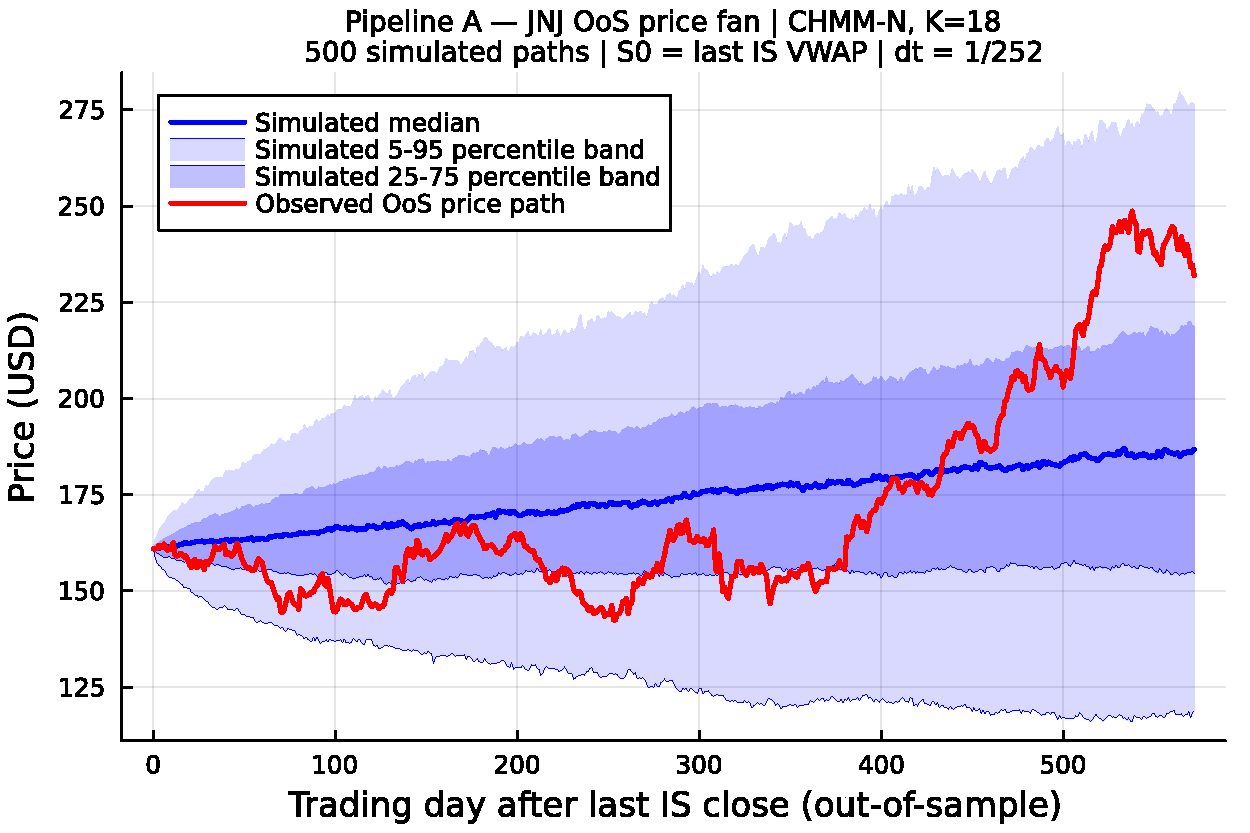
\includegraphics[width=\textwidth]{figs/Fig-JNJ-PriceFan-N.pdf}
    \caption{CHMM-N.}
\end{subfigure}
\begin{subfigure}[t]{0.32\textwidth}
    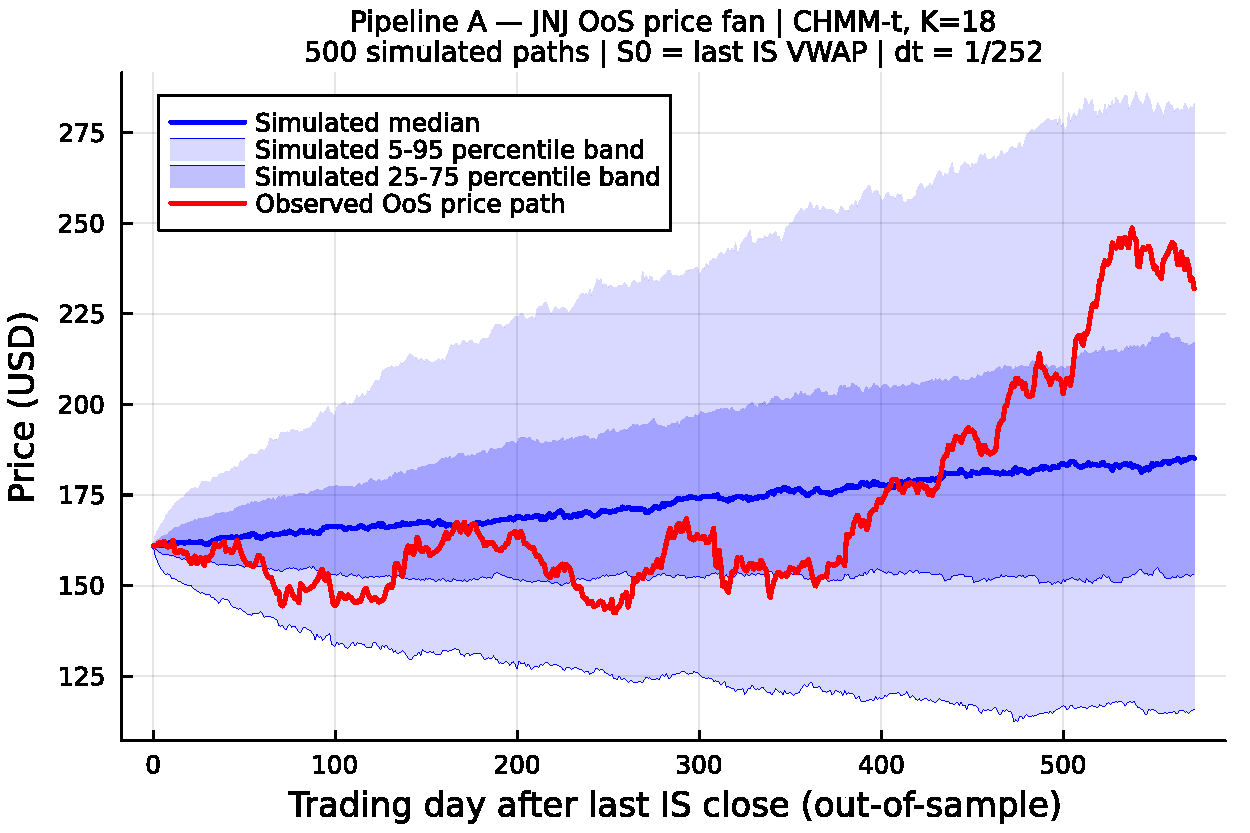
\includegraphics[width=\textwidth]{figs/Fig-JNJ-PriceFan-t.pdf}
    \caption{CHMM-t.}
\end{subfigure}
\begin{subfigure}[t]{0.32\textwidth}
    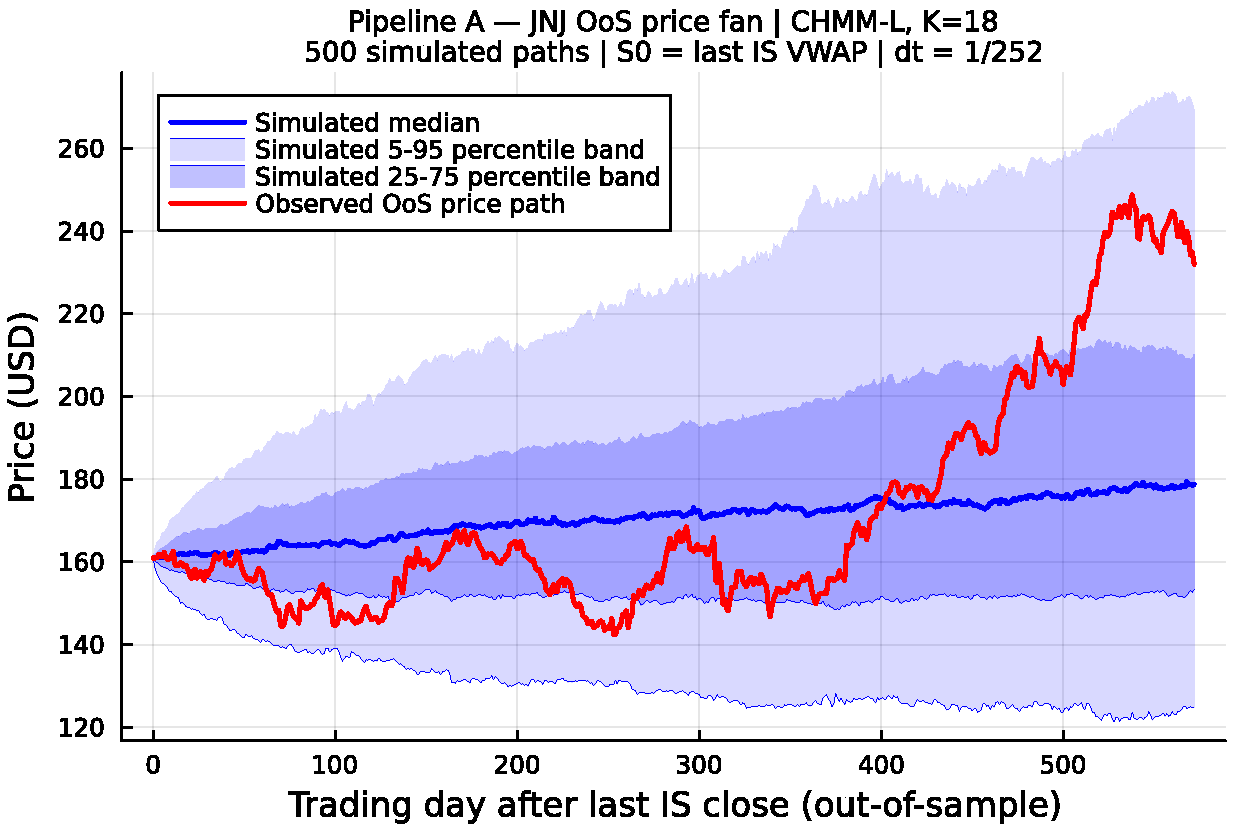
\includegraphics[width=\textwidth]{figs/Fig-JNJ-PriceFan-L.pdf}
    \caption{CHMM-L.}
\end{subfigure}
\caption{JNJ out-of-sample price fan, unconditional CHMM sampler.}
\label{fig:price_fan_jnj_appendix}
\end{figure}

\begin{figure}[h]
\centering
\begin{subfigure}[t]{0.32\textwidth}
    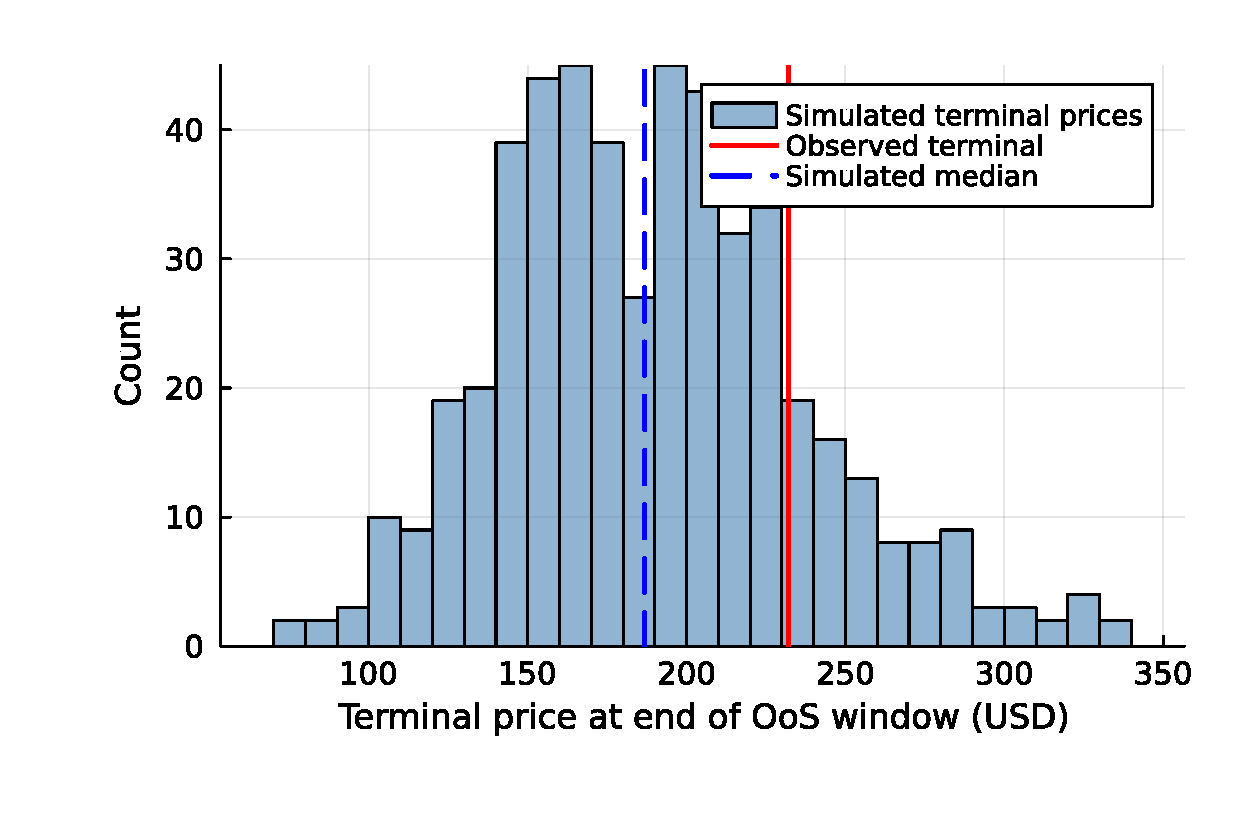
\includegraphics[width=\textwidth]{figs/Fig-JNJ-TerminalDist-N.pdf}
    \caption{CHMM-N.}
\end{subfigure}
\begin{subfigure}[t]{0.32\textwidth}
    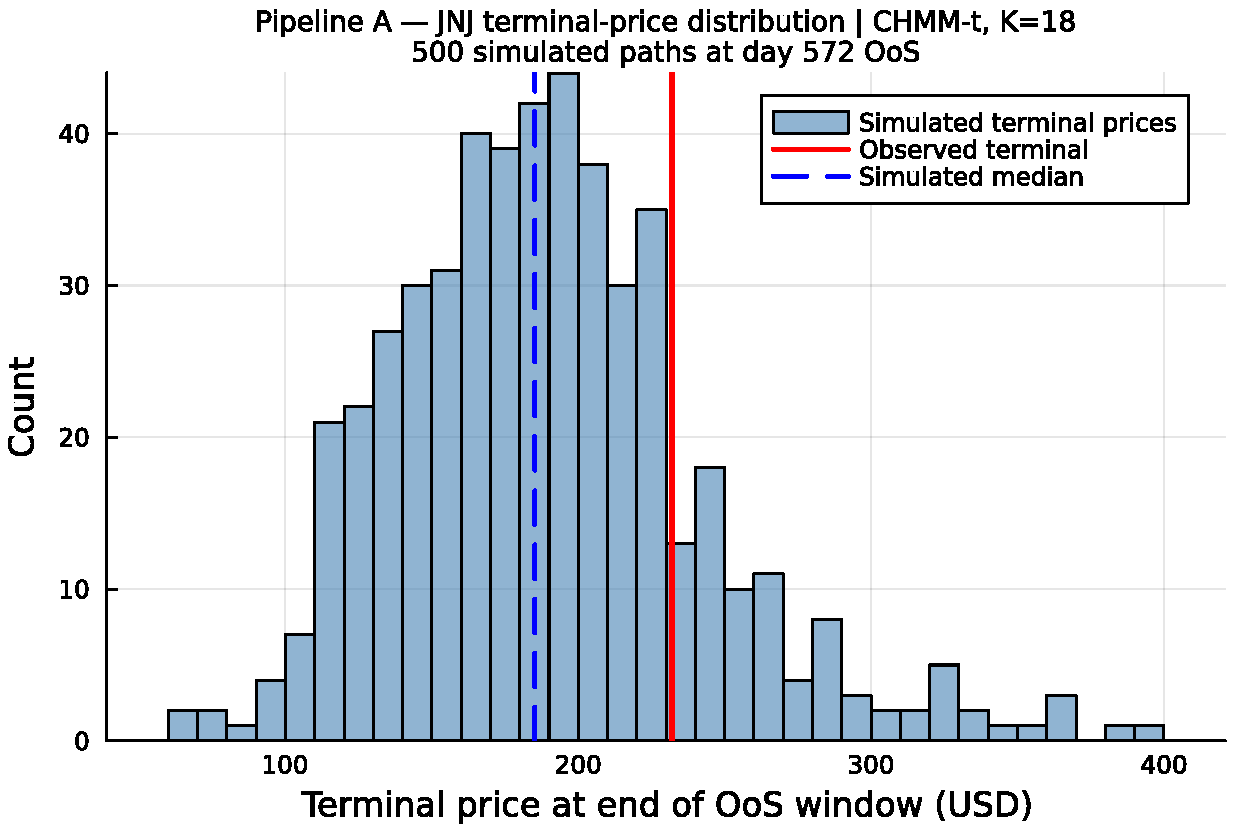
\includegraphics[width=\textwidth]{figs/Fig-JNJ-TerminalDist-t.pdf}
    \caption{CHMM-t.}
\end{subfigure}
\begin{subfigure}[t]{0.32\textwidth}
    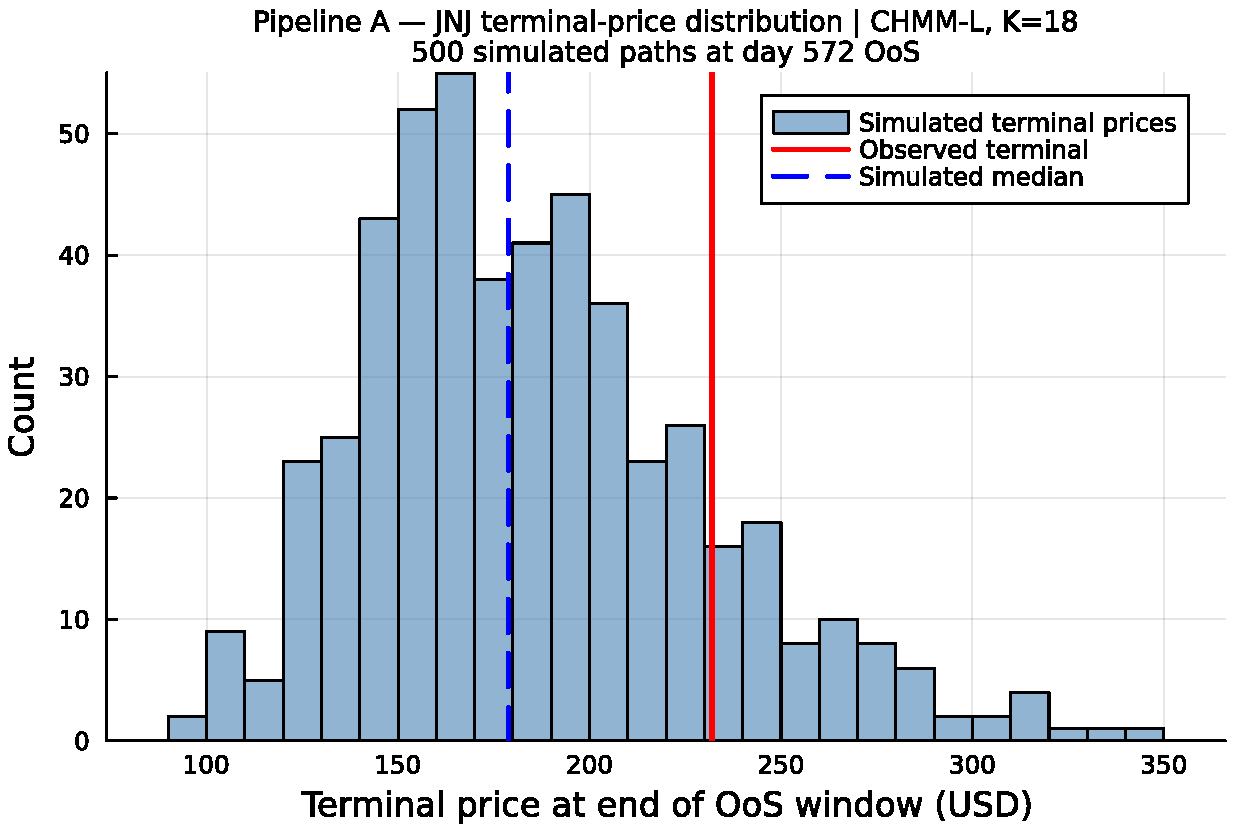
\includegraphics[width=\textwidth]{figs/Fig-JNJ-TerminalDist-L.pdf}
    \caption{CHMM-L.}
\end{subfigure}
\caption{JNJ terminal-price distribution, unconditional CHMM sampler.}
\label{fig:terminal_jnj_appendix}
\end{figure}

\begin{figure}[h]
\centering
\begin{subfigure}[t]{0.32\textwidth}
    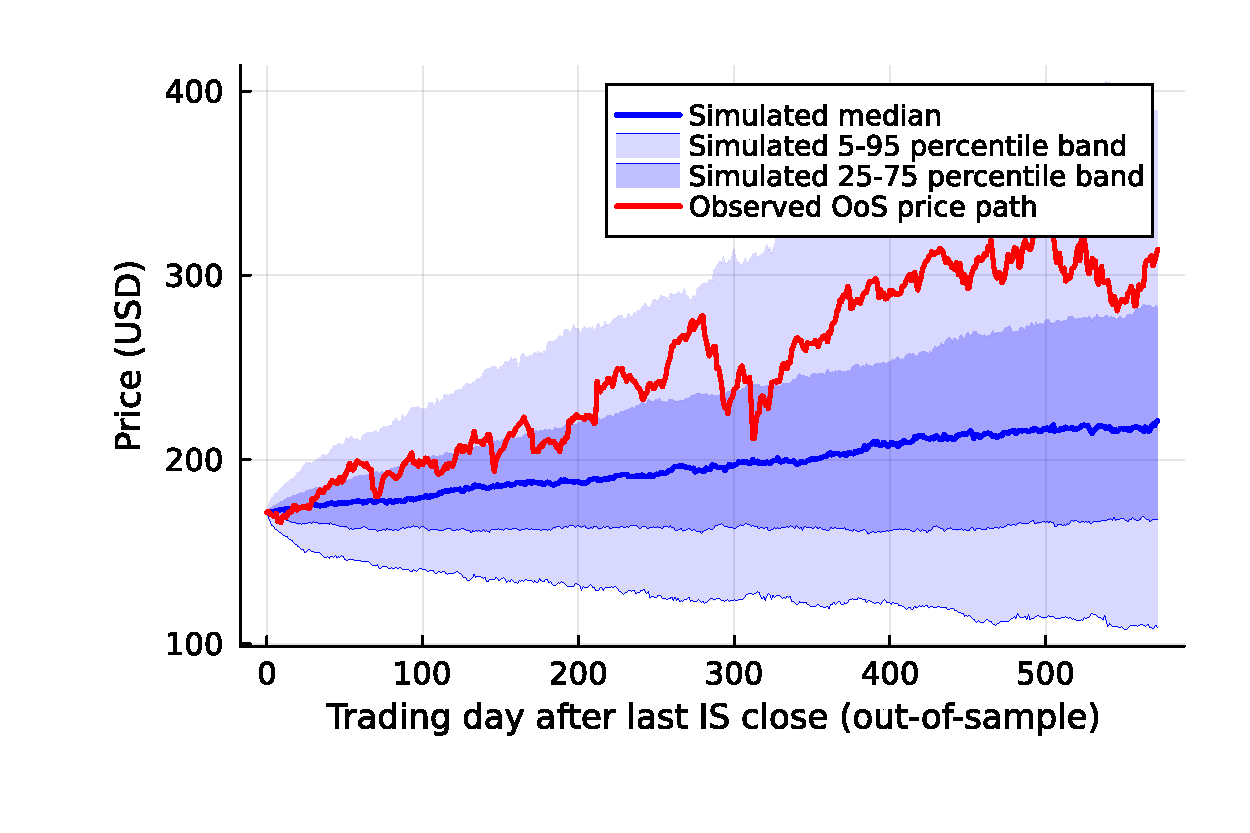
\includegraphics[width=\textwidth]{figs/Fig-JPM-PriceFan-N.pdf}
    \caption{CHMM-N.}
\end{subfigure}
\begin{subfigure}[t]{0.32\textwidth}
    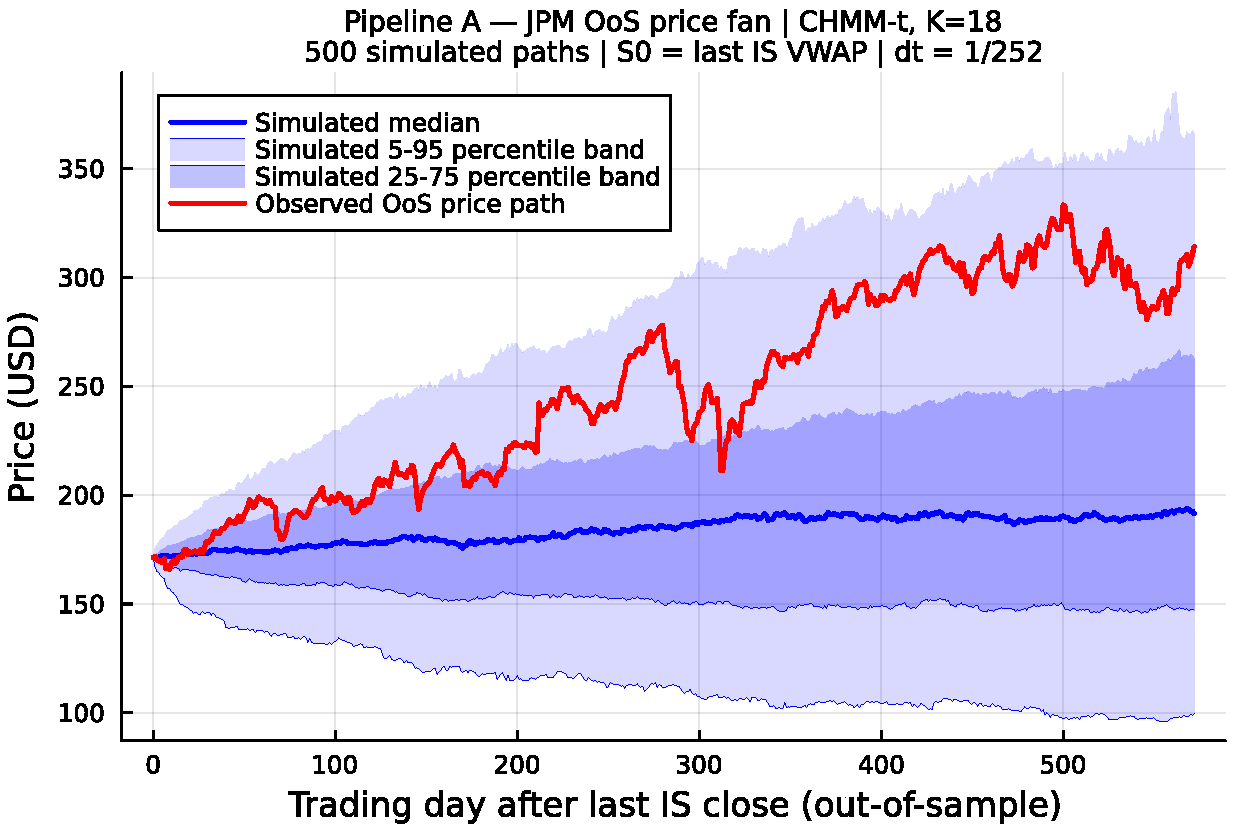
\includegraphics[width=\textwidth]{figs/Fig-JPM-PriceFan-t.pdf}
    \caption{CHMM-t.}
\end{subfigure}
\begin{subfigure}[t]{0.32\textwidth}
    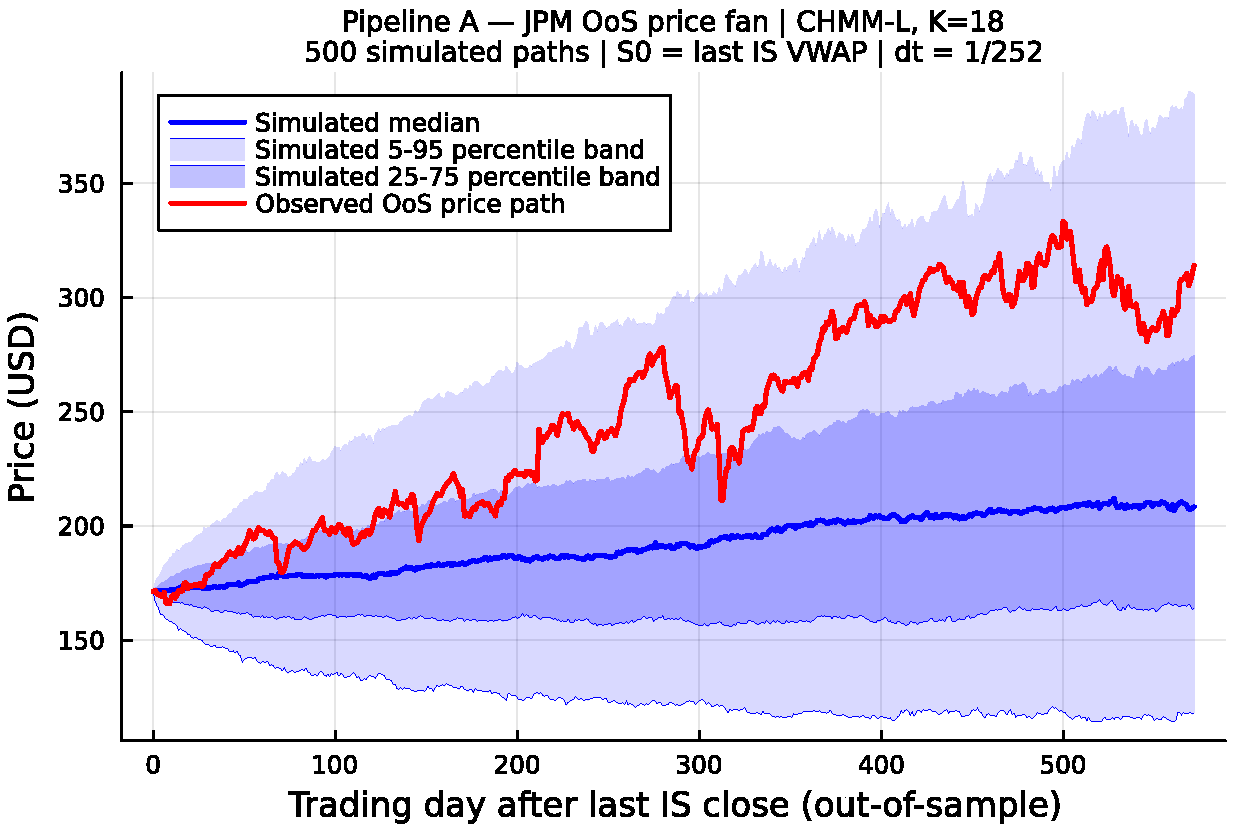
\includegraphics[width=\textwidth]{figs/Fig-JPM-PriceFan-L.pdf}
    \caption{CHMM-L.}
\end{subfigure}
\caption{JPM out-of-sample price fan, unconditional CHMM sampler.}
\label{fig:price_fan_jpm_appendix}
\end{figure}

\begin{figure}[h]
\centering
\begin{subfigure}[t]{0.32\textwidth}
    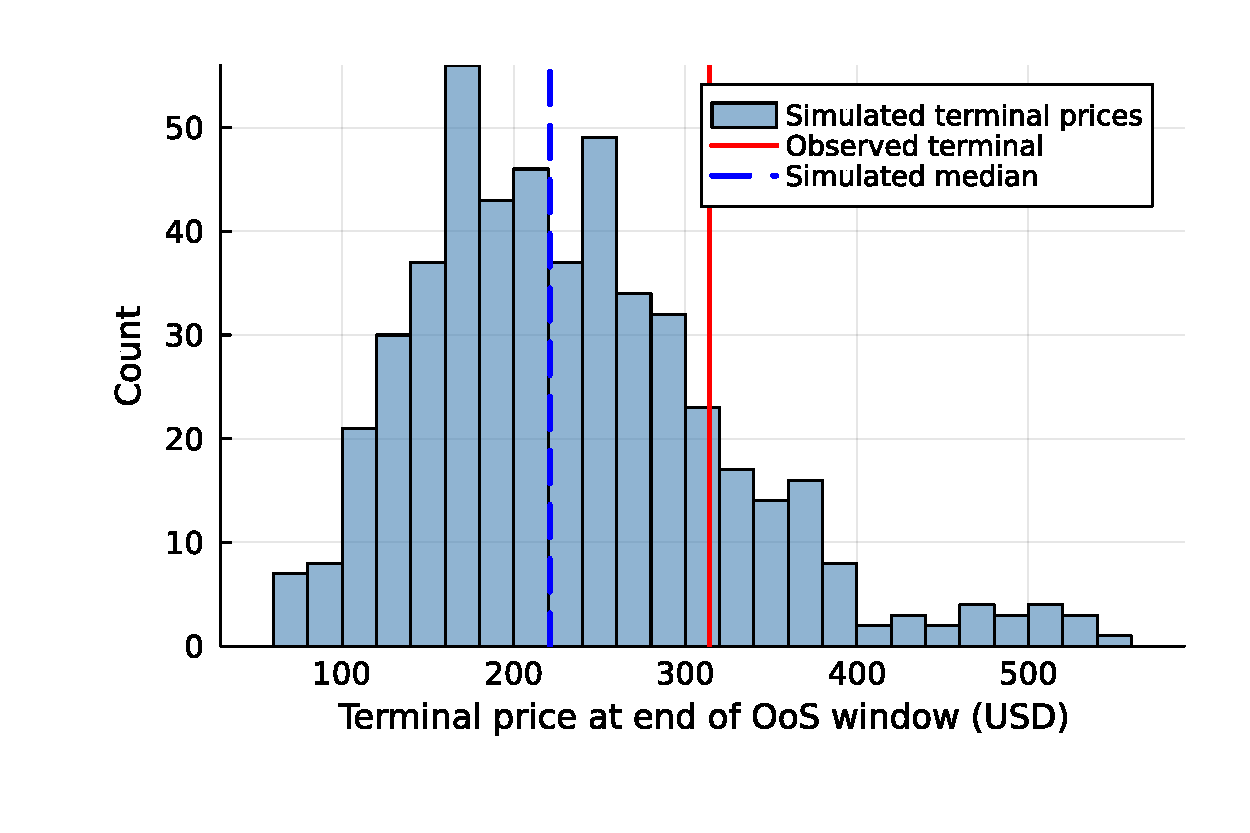
\includegraphics[width=\textwidth]{figs/Fig-JPM-TerminalDist-N.pdf}
    \caption{CHMM-N.}
\end{subfigure}
\begin{subfigure}[t]{0.32\textwidth}
    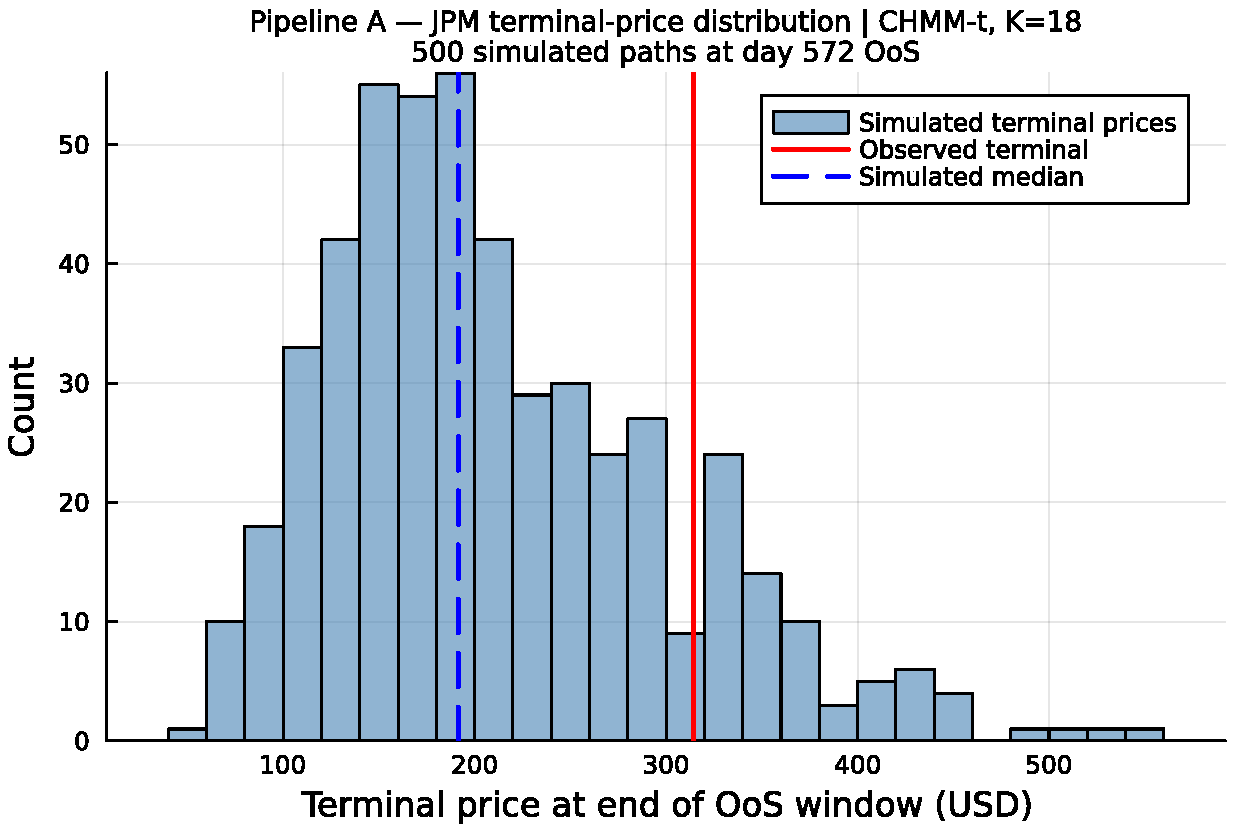
\includegraphics[width=\textwidth]{figs/Fig-JPM-TerminalDist-t.pdf}
    \caption{CHMM-t.}
\end{subfigure}
\begin{subfigure}[t]{0.32\textwidth}
    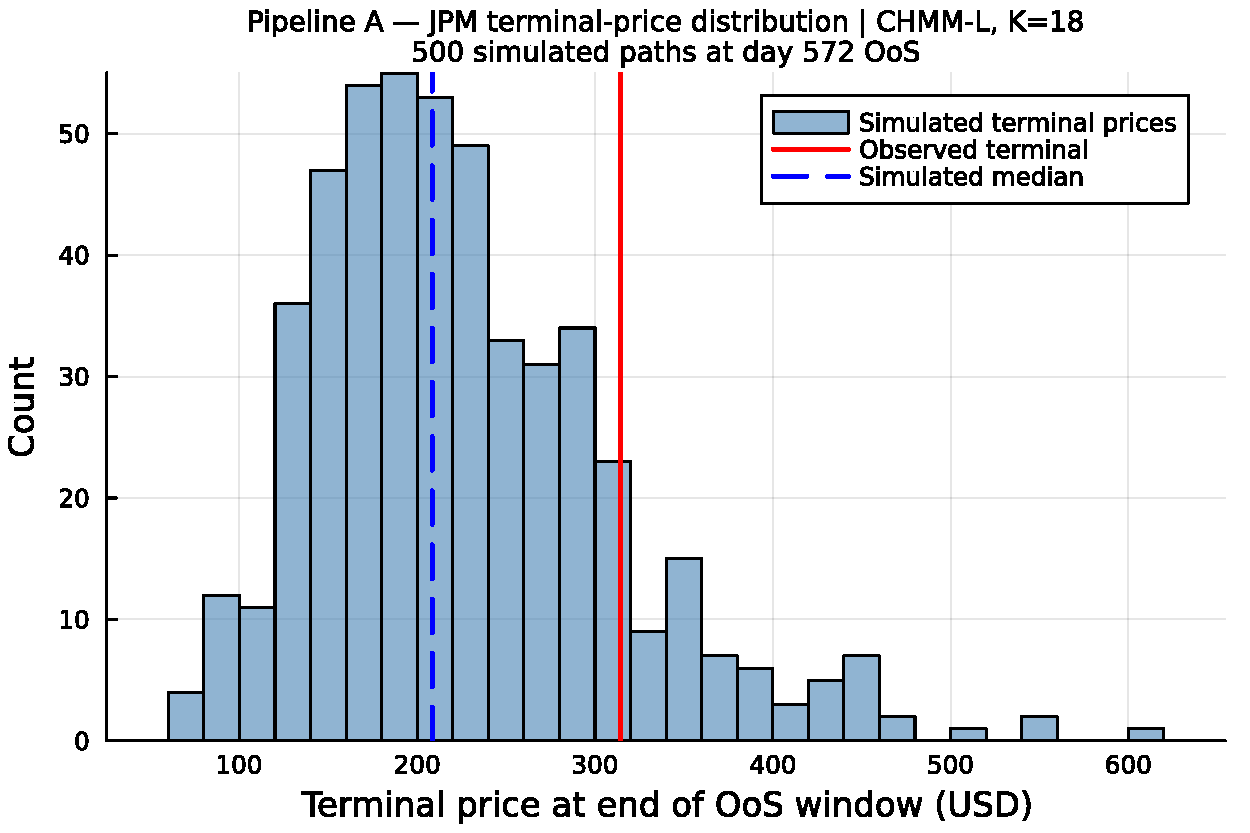
\includegraphics[width=\textwidth]{figs/Fig-JPM-TerminalDist-L.pdf}
    \caption{CHMM-L.}
\end{subfigure}
\caption{JPM terminal-price distribution, unconditional CHMM sampler.}
\label{fig:terminal_jpm_appendix}
\end{figure}

\begin{figure}[h]
\centering
\begin{subfigure}[t]{0.32\textwidth}
    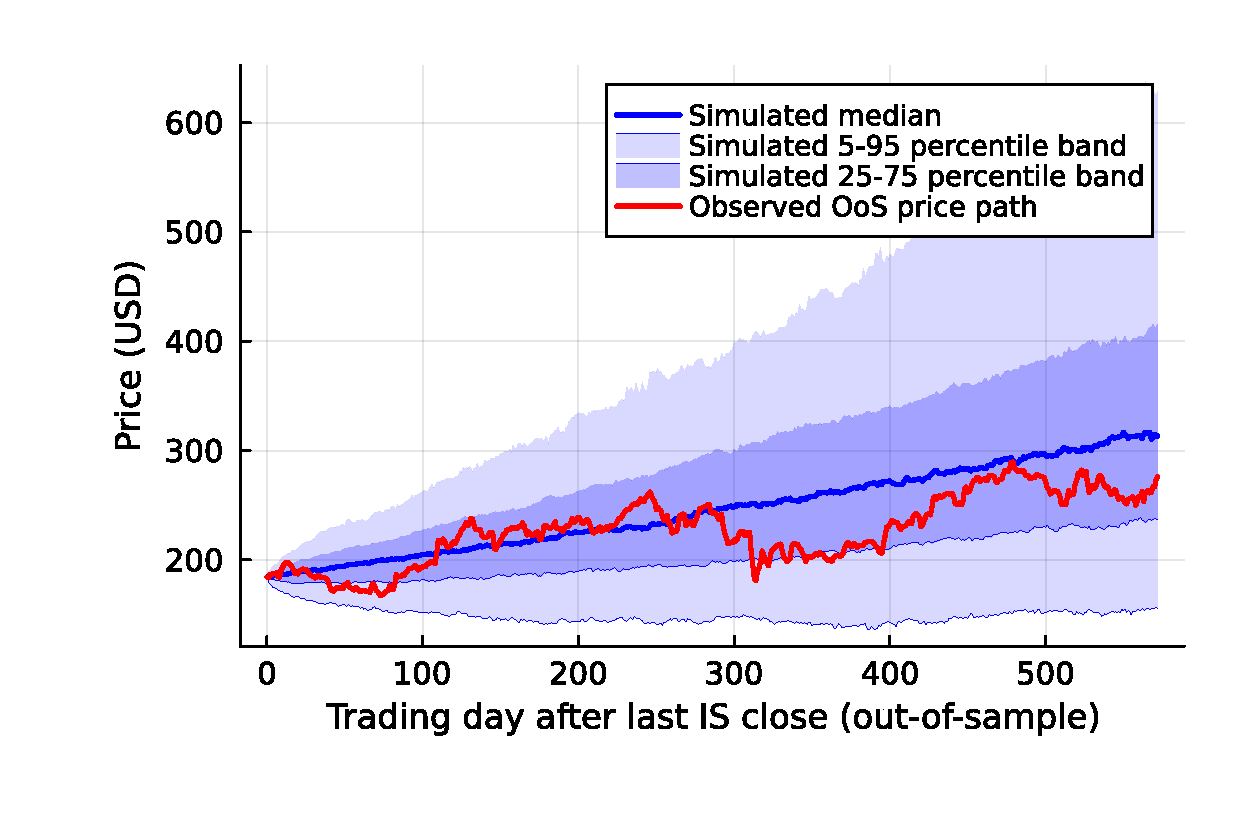
\includegraphics[width=\textwidth]{figs/Fig-AAPL-PriceFan-N.pdf}
    \caption{CHMM-N.}
\end{subfigure}
\begin{subfigure}[t]{0.32\textwidth}
    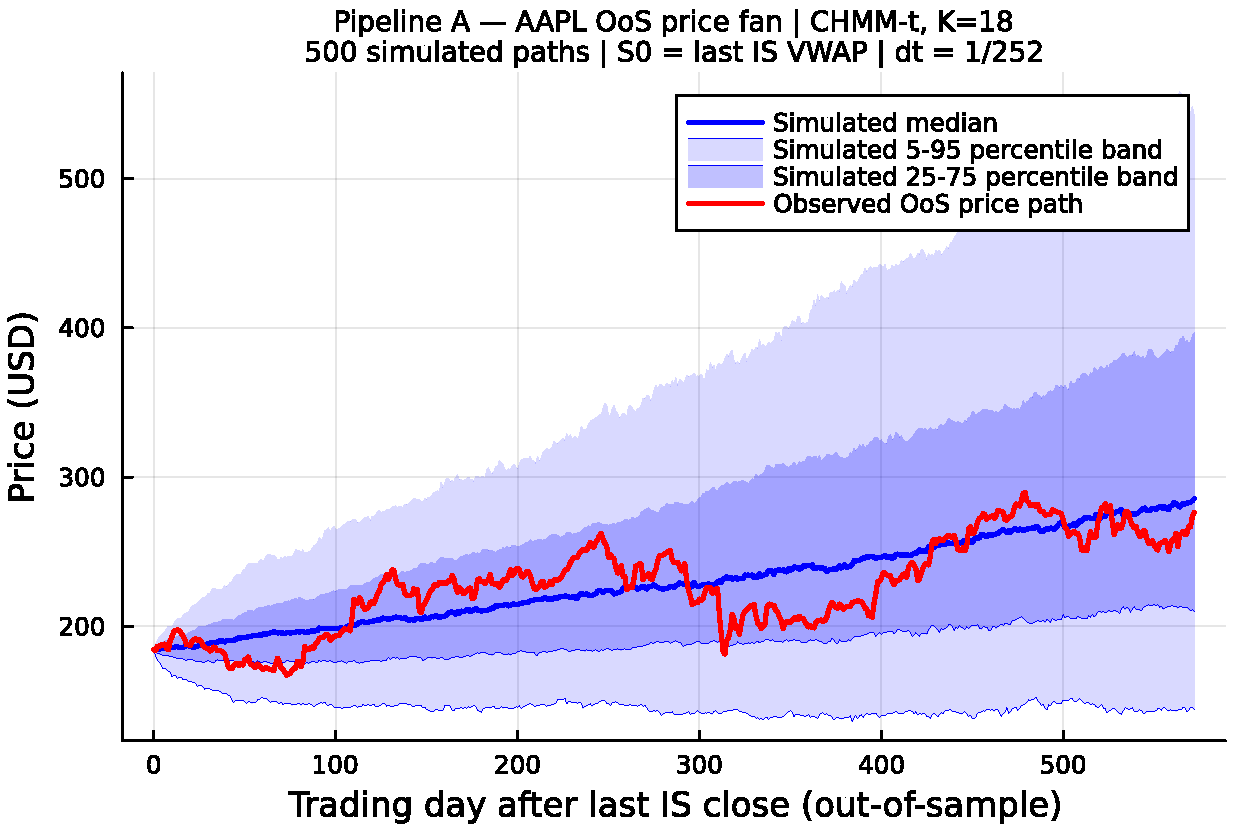
\includegraphics[width=\textwidth]{figs/Fig-AAPL-PriceFan-t.pdf}
    \caption{CHMM-t.}
\end{subfigure}
\begin{subfigure}[t]{0.32\textwidth}
    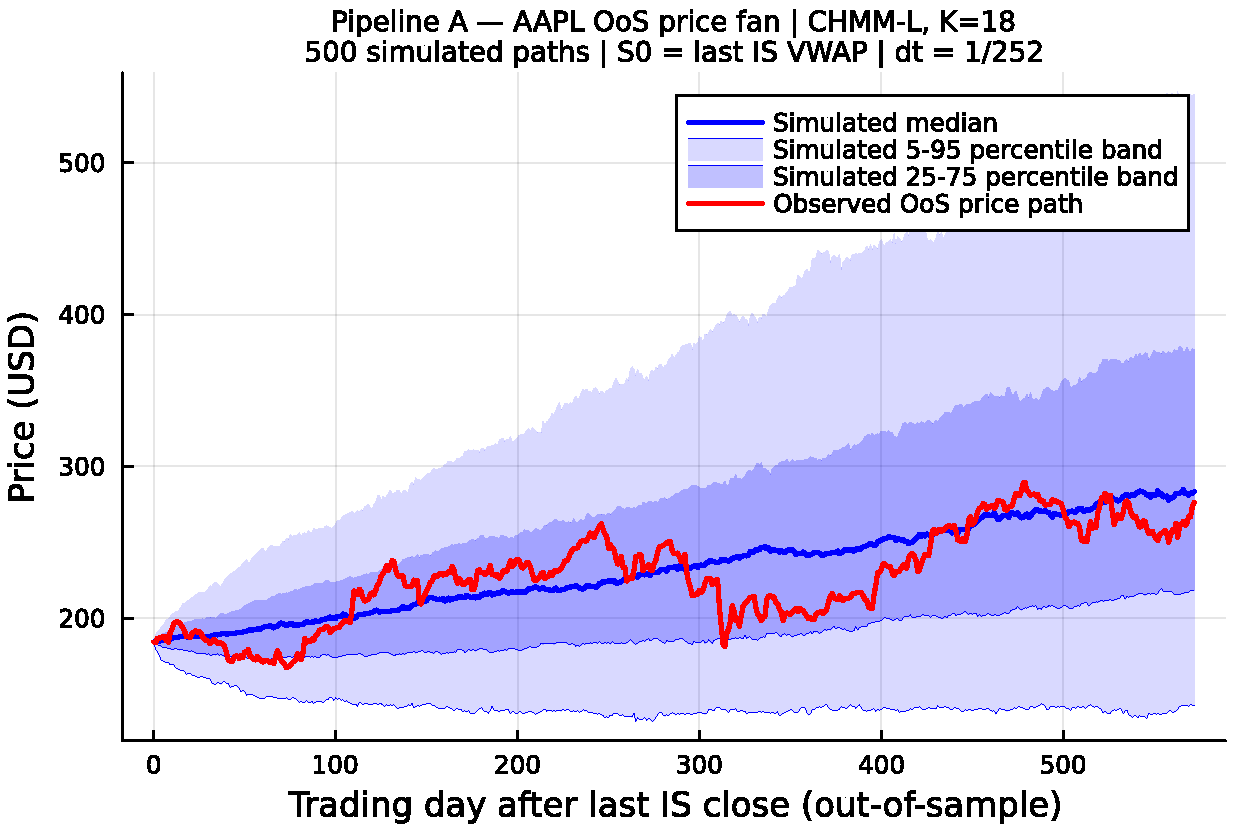
\includegraphics[width=\textwidth]{figs/Fig-AAPL-PriceFan-L.pdf}
    \caption{CHMM-L.}
\end{subfigure}
\caption{AAPL out-of-sample price fan, unconditional CHMM sampler.}
\label{fig:price_fan_aapl_appendix}
\end{figure}

\begin{figure}[h]
\centering
\begin{subfigure}[t]{0.32\textwidth}
    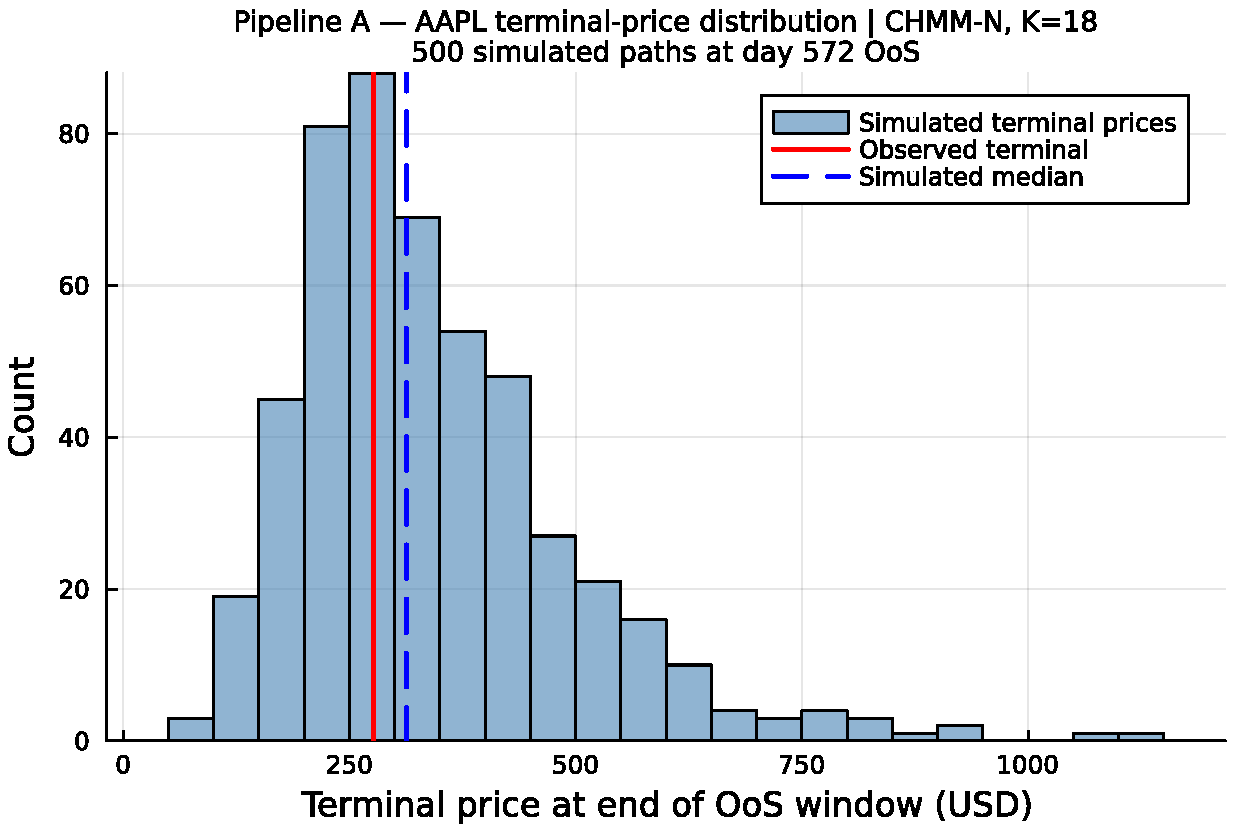
\includegraphics[width=\textwidth]{figs/Fig-AAPL-TerminalDist-N.pdf}
    \caption{CHMM-N.}
\end{subfigure}
\begin{subfigure}[t]{0.32\textwidth}
    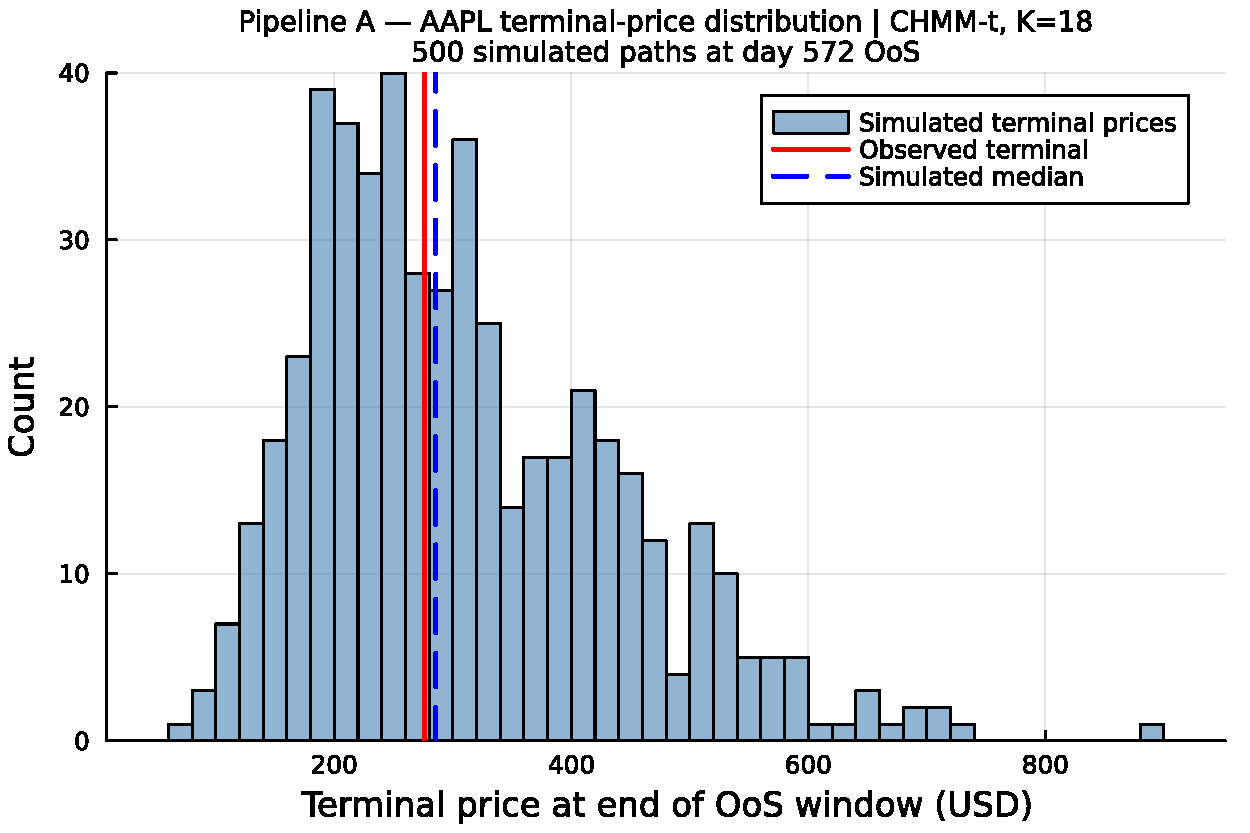
\includegraphics[width=\textwidth]{figs/Fig-AAPL-TerminalDist-t.pdf}
    \caption{CHMM-t.}
\end{subfigure}
\begin{subfigure}[t]{0.32\textwidth}
    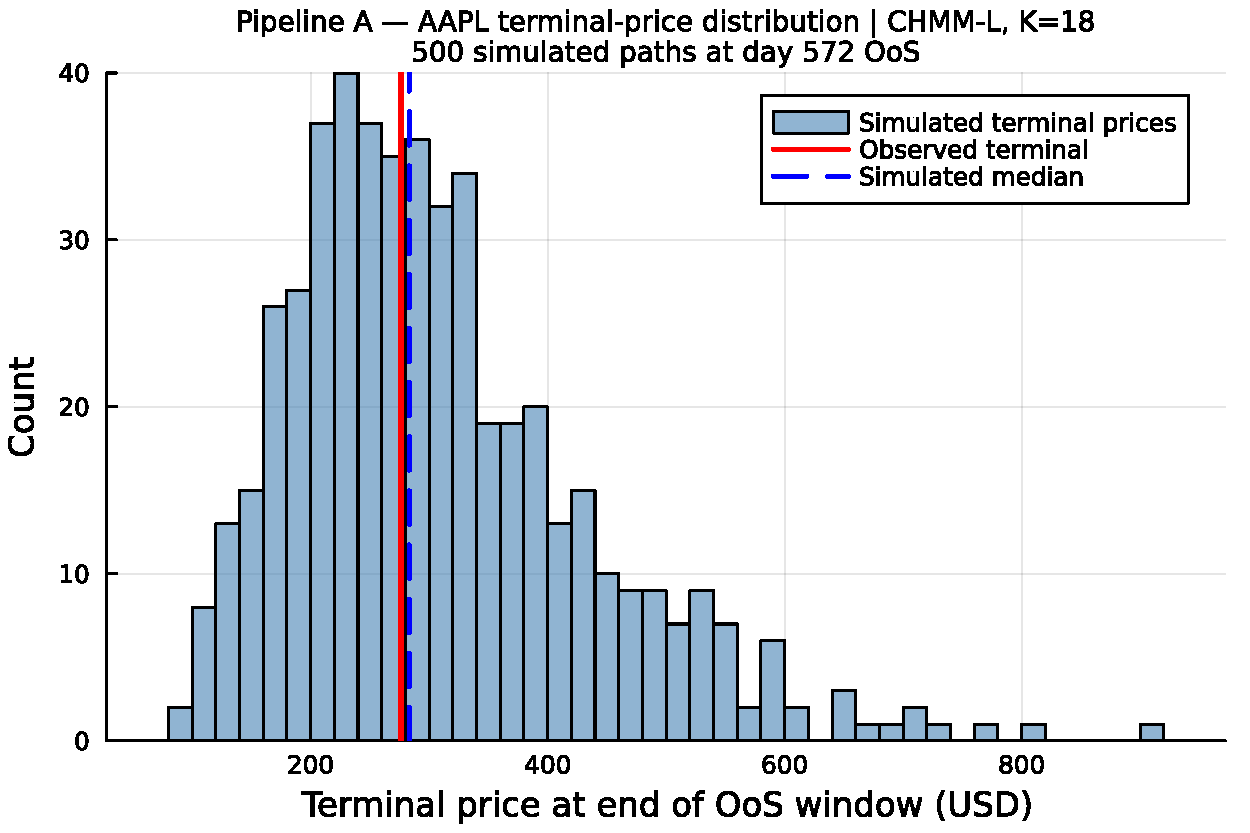
\includegraphics[width=\textwidth]{figs/Fig-AAPL-TerminalDist-L.pdf}
    \caption{CHMM-L.}
\end{subfigure}
\caption{AAPL terminal-price distribution, unconditional CHMM sampler.}
\label{fig:terminal_aapl_appendix}
\end{figure}

\begin{figure}[h]
\centering
\begin{subfigure}[t]{0.32\textwidth}
    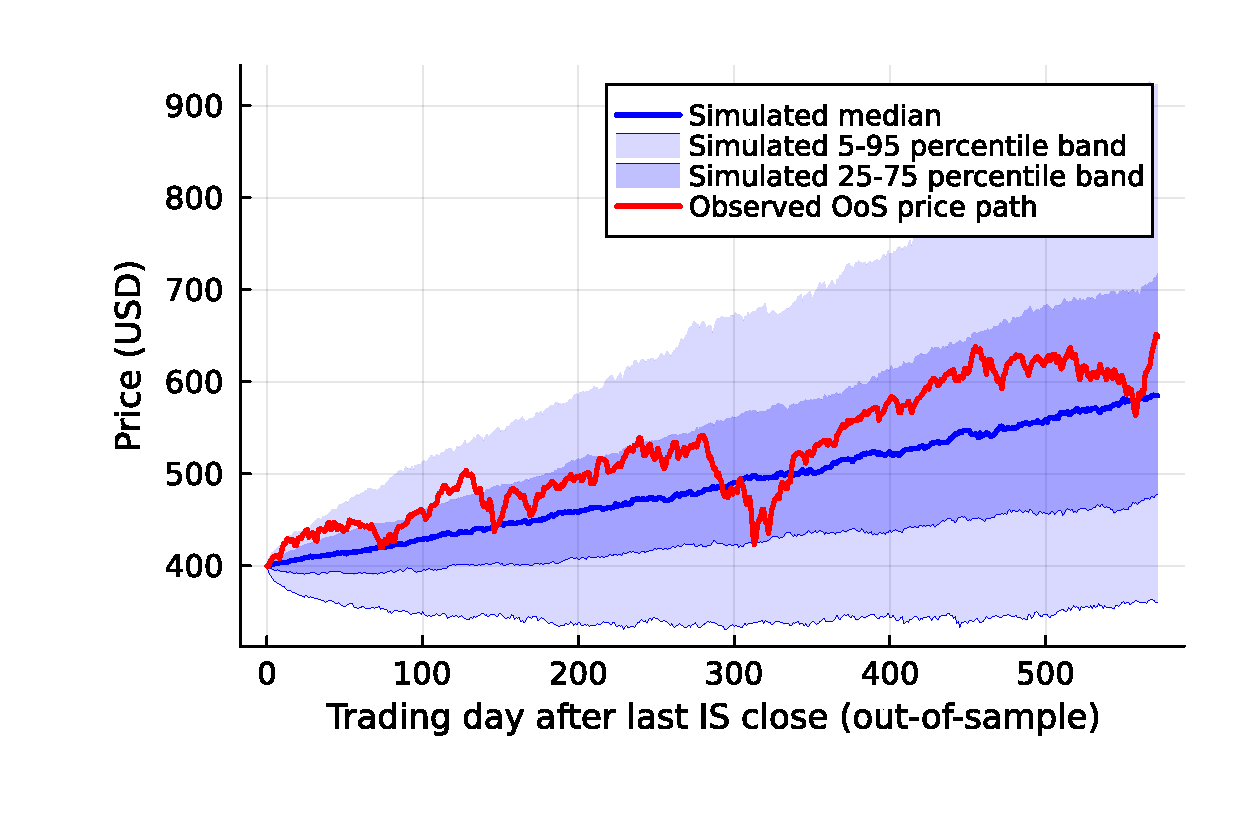
\includegraphics[width=\textwidth]{figs/Fig-QQQ-PriceFan-N.pdf}
    \caption{CHMM-N.}
\end{subfigure}
\begin{subfigure}[t]{0.32\textwidth}
    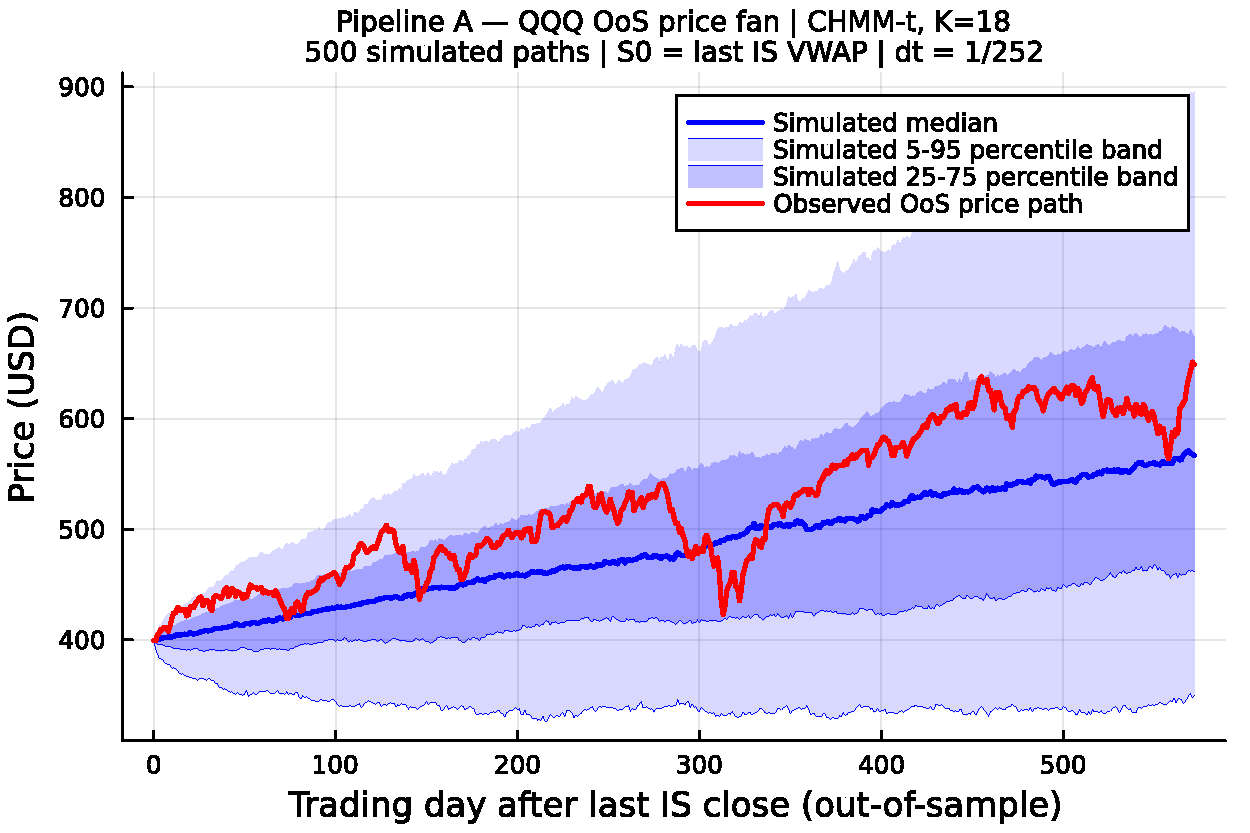
\includegraphics[width=\textwidth]{figs/Fig-QQQ-PriceFan-t.pdf}
    \caption{CHMM-t.}
\end{subfigure}
\begin{subfigure}[t]{0.32\textwidth}
    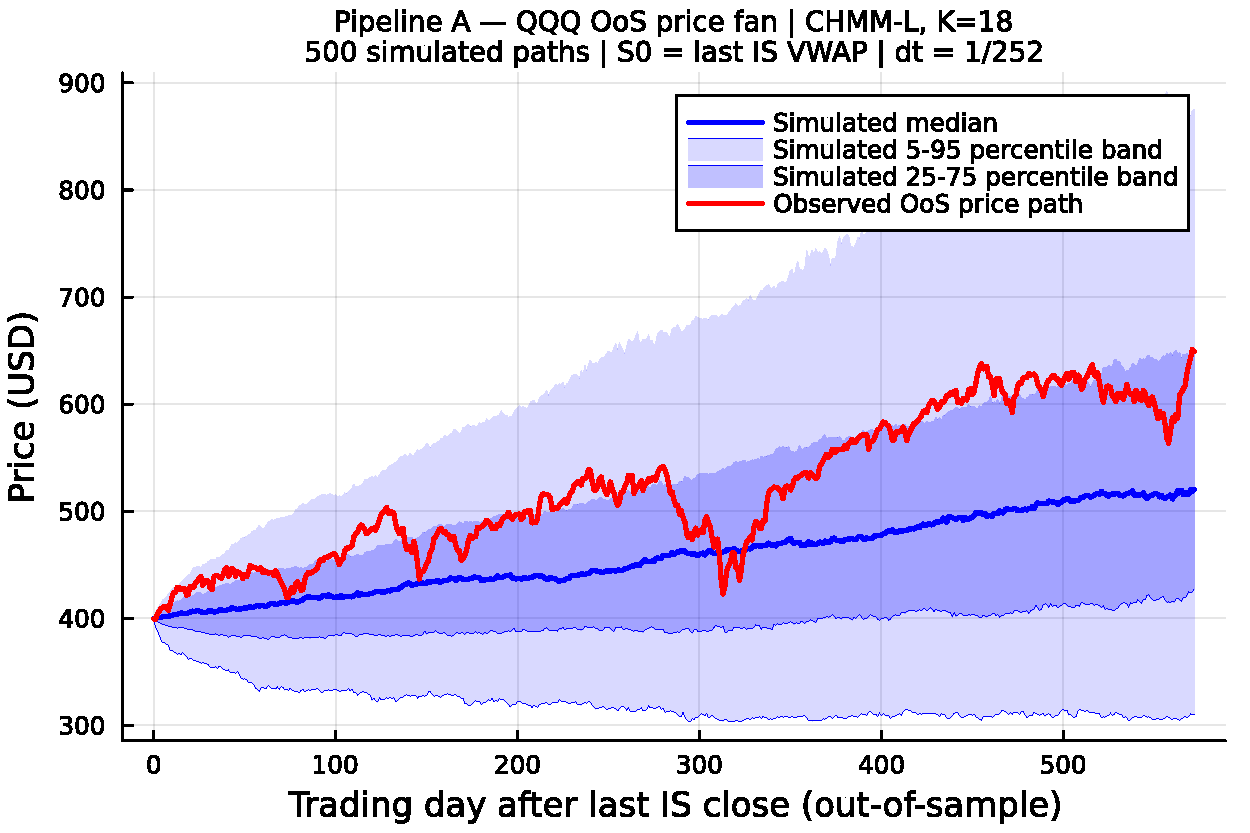
\includegraphics[width=\textwidth]{figs/Fig-QQQ-PriceFan-L.pdf}
    \caption{CHMM-L.}
\end{subfigure}
\caption{QQQ out-of-sample price fan, unconditional CHMM sampler.}
\label{fig:price_fan_qqq_appendix}
\end{figure}

\begin{figure}[h]
\centering
\begin{subfigure}[t]{0.32\textwidth}
    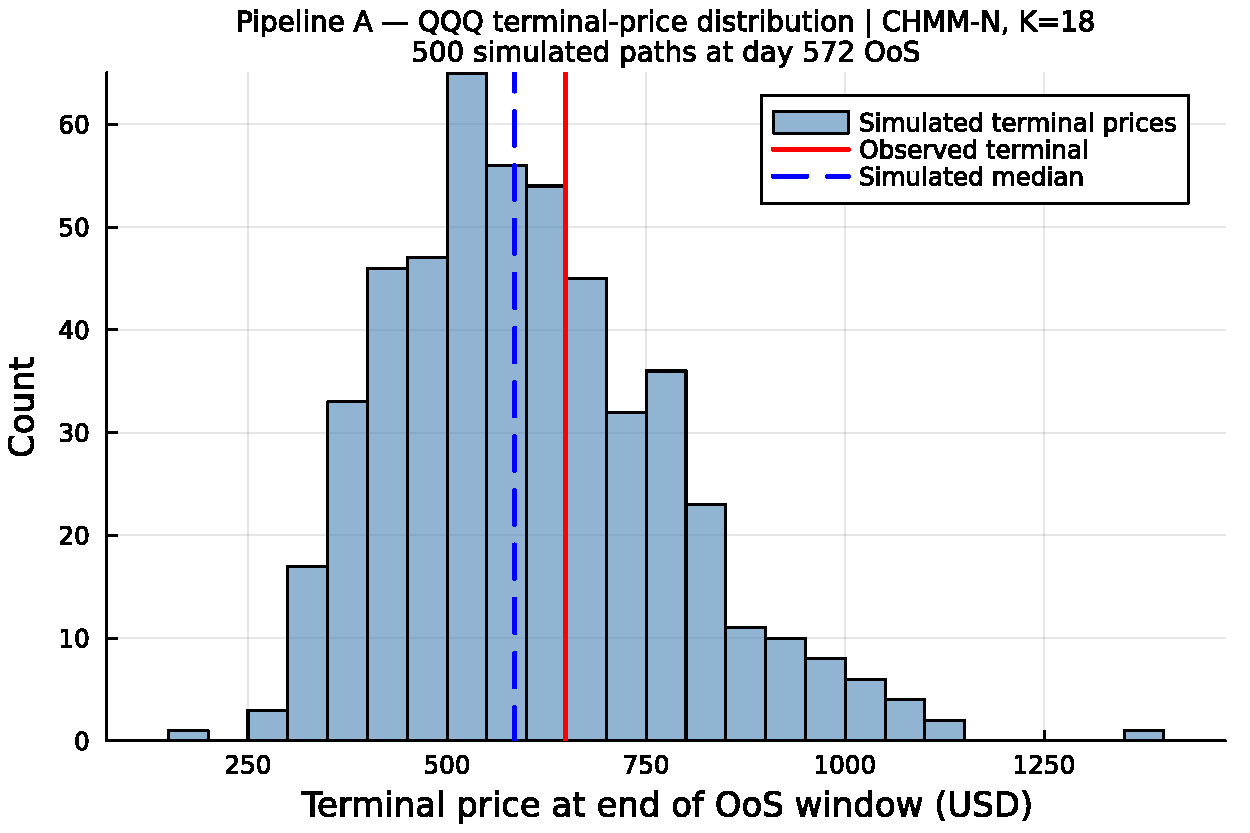
\includegraphics[width=\textwidth]{figs/Fig-QQQ-TerminalDist-N.pdf}
    \caption{CHMM-N.}
\end{subfigure}
\begin{subfigure}[t]{0.32\textwidth}
    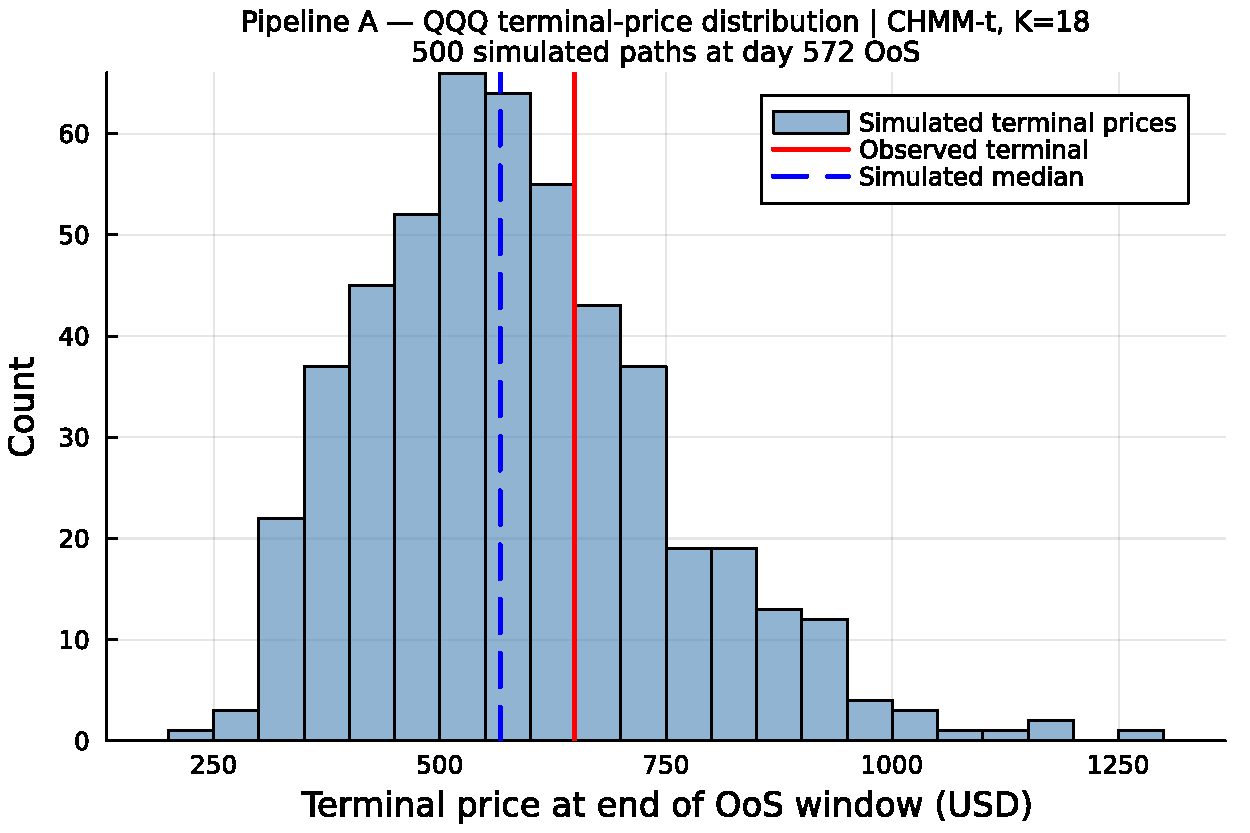
\includegraphics[width=\textwidth]{figs/Fig-QQQ-TerminalDist-t.pdf}
    \caption{CHMM-t.}
\end{subfigure}
\begin{subfigure}[t]{0.32\textwidth}
    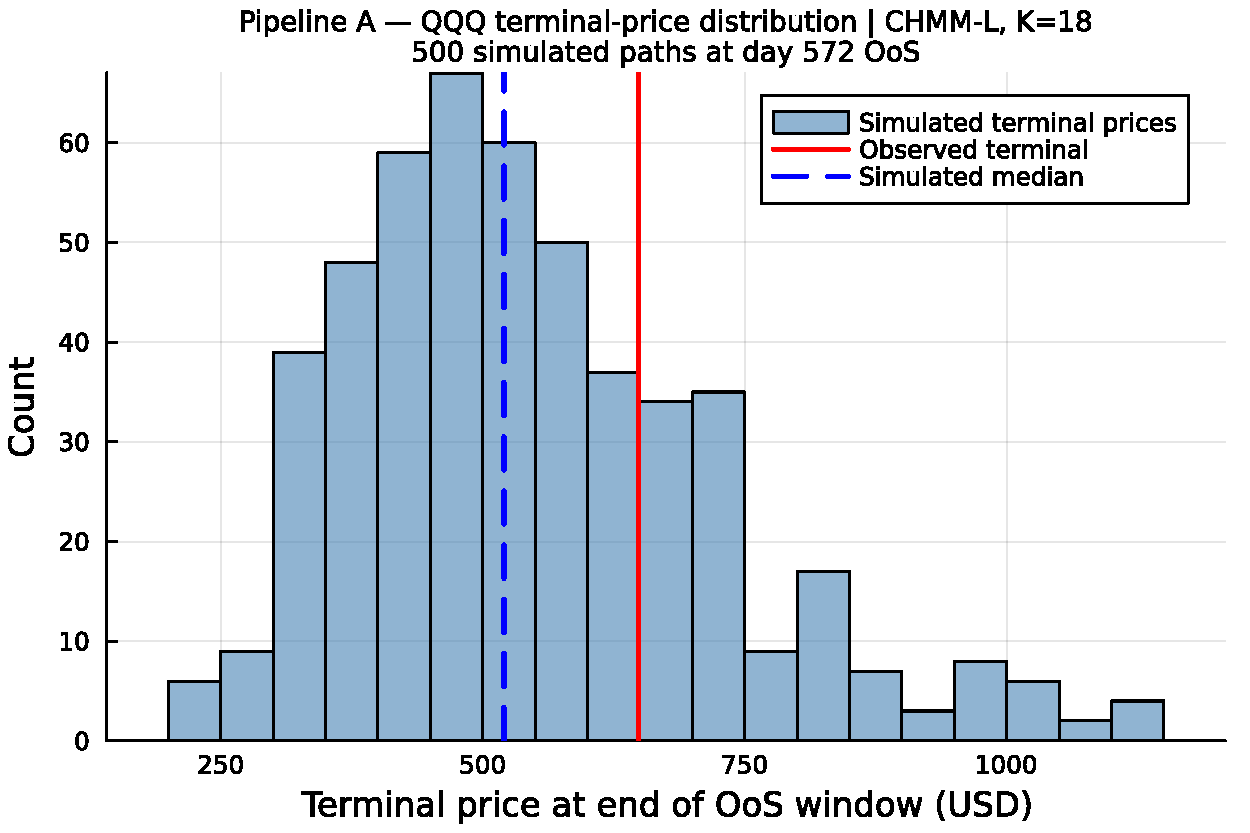
\includegraphics[width=\textwidth]{figs/Fig-QQQ-TerminalDist-L.pdf}
    \caption{CHMM-L.}
\end{subfigure}
\caption{QQQ terminal-price distribution, unconditional CHMM sampler.}
\label{fig:terminal_qqq_appendix}
\end{figure}


